\chapter{Discussion}
\label{chap:discussion}

Chapter~\ref{chap:results} reported the empirical results. This chapter
interprets them: how the headline outcomes fit the design intent of
Chapter~\ref{chap:methodology}, how the memory and orchestration
comparisons should be read, and how the cost picture compares with
practical alternatives. The Limitations subsection summarises the
boundaries; the Conclusion in Chapter~\ref{chap:conclusion} returns to
the original research question and hypothesis with these
interpretations in hand.

% ─────────────────────────────────────────────────────────────────────────────
\section{Interpretation of the Headline Outcomes}
\label{sec:discussion_headline}
% ─────────────────────────────────────────────────────────────────────────────

The results show that the system can usually place the target disease,
or a closely related disease, in the differential diagnosis. The
combined found rate is $94.4\,\%$ (151/160) on the 160-patient paired
cohort under the principal multi-level memory configuration, and the
correct or related condition is ranked first in $64.5\,\%$ of found
cases (Rank-1 within found). The pipeline also completed without any
full patient-run aborts. This supports the main design choice of the
thesis: a coordinated workflow of specialised agents is more
inspectable and reliable than asking one model to do the whole task
in one call. The Section~\ref{sec:results_single_llm} single-LLM
controlled baseline attaches a number to that claim --- the
multi-agent orchestration buys $+33.8$ percentage points on DIRECT
and $+20.0$ percentage points on Found over a single-call
configuration on the same 160 patients with the same reasoning model.

% ─────────────────────────────────────────────────────────────────────────────
\section{Interpretation of the Memory A/B}
\label{sec:discussion_memory}
% ─────────────────────────────────────────────────────────────────────────────

The memory result is large on the paired controlled comparison. The
principal multi-level memory configuration lifts DIRECT from
\textbf{$53.8\,\%$} (86/160, the single-level baseline) to
\textbf{$76.9\,\%$} (123/160) on the same 160 patients, a
$+23.1$ percentage-point gain. The Found rate moves in the same
direction ($+1.9$ pp, $92.5\,\% \to 94.4\,\%$), with a matching
drop on MISS. The qualitative pattern in the case walkthroughs of
Section~\ref{sec:results_qualitative} is consistent with this: the
case-based prior surfaces clinically similar past patients in the
Diagnostic Reasoning agent's working memory, broadening the
differential and lifting the rank-1 commitment toward the
clinically-defensible most-specific term when the evidence supports
it.

% ─────────────────────────────────────────────────────────────────────────────
\section{Model Comparison Read}
\label{sec:discussion_model}
% ─────────────────────────────────────────────────────────────────────────────

The model comparison matters for practical use. On the same
20-patient subset, GPT-OSS-120B served via Groq runs about
$13\times$ faster than Med42-70B served locally on Ollama (median
$\sim$108\,s vs.\ $\sim$2\,000\,s per patient) and also delivers a
higher DIRECT rate ($40\,\%$ vs.\ $25\,\%$, 8/20 vs.\ 5/20). For a
doctor using the system as a runtime second opinion the wall-clock
gap is the dominant finding: a clinician cannot wait half an hour
per patient, and the latency gap is several orders of magnitude
larger than the per-patient runtime noise. In a multi-agent
pipeline, every extra model call adds time, so inference speed is
not a minor implementation detail; it affects whether the system can
be used interactively.

% ─────────────────────────────────────────────────────────────────────────────
\section{Token and Cost Accounting}
\label{sec:discussion_cost}
% ─────────────────────────────────────────────────────────────────────────────

The LLM adapter does not currently persist token counts, so direct
per-patient token consumption is not reported. A first-order cost
estimate can still be derived from the persisted agent outputs and the
input case files: averaging across the 160-patient cohort, each
patient run uses an estimated 80--90~k input tokens and 18--22~k
output tokens spread across the seven agents, with the Diagnostic
Reasoning agent dominating because of its multi-round adaptive loop.
At Groq's published rates (GPT-OSS-120B at \$0.15 / M input, \$0.75 /
M output; Qwen3-32B at \$0.29 / M input, \$0.59 / M output) this
gives an estimated cost of \textbf{approximately \$0.03 per patient
run} (reasonable range \$0.01--\$0.04 depending on diagnostic-round
count and treatment-planning eligibility). At this rate, the
160-patient cohort cost approximately \$5; a 1{,}000-patient
evaluation would cost approximately \$30. The estimate excludes
embedding and Qdrant infrastructure costs (both negligible at this
scale) and is conservative on the input side because the Diagnostic
Reasoning loop's intermediate-call inputs are not separately
persisted. Direct token instrumentation in the LLM adapter is
identified as future work; once added, the estimate above can be
replaced with measured numbers per patient.

% ─────────────────────────────────────────────────────────────────────────────
\section{Clinical Workflow Integration}
\label{sec:discussion_workflow}
% ─────────────────────────────────────────────────────────────────────────────

\begin{figure}[ht]
  \centering
  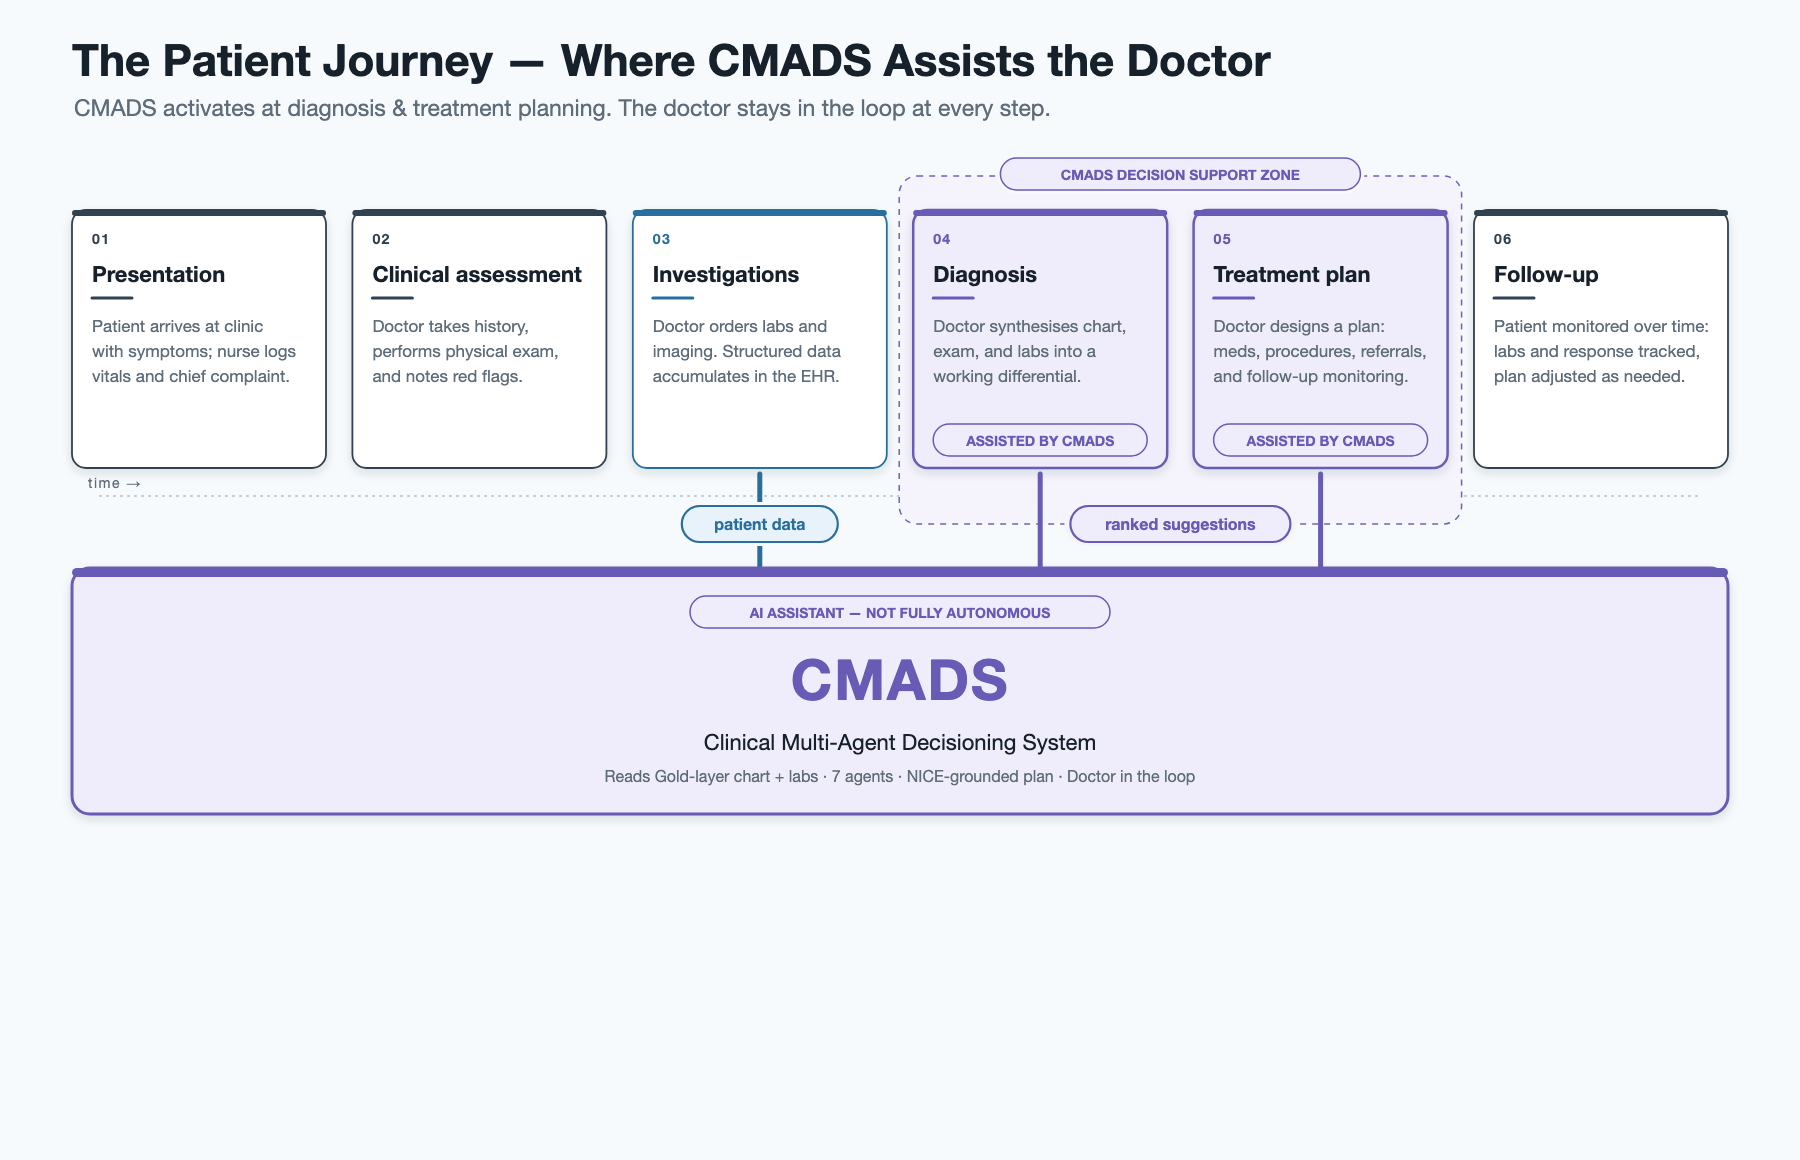
\includegraphics[width=\linewidth]{images/ch1_patient_journey.png}
  \caption[The patient journey alongside CMADS]{The patient journey through
    a consultation, with CMADS positioned as an assistive layer at the
    diagnosis and treatment-plan stages. Structured chart and lab data
    flow into the system after investigations; the system returns a
    ranked differential and a guideline-grounded plan. The doctor is in
    the loop for every CMADS-assisted step.}
  \label{fig:patient_journey}
\end{figure}

The headline numbers in Section~\ref{sec:discussion_headline} only
matter if the system can plausibly sit inside a real consultation.
Figure~\ref{fig:patient_journey} sketches the intended interaction
shape: investigations accumulate structured data in the EHR, CMADS
reads the same Gold-layer JSON, and a ranked top-5 differential plus a
plan is surfaced back to the doctor for review.
The intended interaction shape is narrow and additive rather than
replacement. A physician opens the doctor-facing console, enters a
patient UUID (or, in a future deployment, uploads a Gold-layer dump
exported from the hospital's EHR), and waits the
approximately two-minute median latency reported in
Section~\ref{sec:results_e2e} for the seven agents to complete. The
console then renders the ranked top-five differential alongside the
agents' reasoning trail and, on DIRECT matches, the NICE-grounded
treatment plan. The clinician treats this output as a
\emph{second opinion}: a structured prompt to widen or narrow the
working differential rather than a binding recommendation. If a
surfaced diagnosis is surprising, the console exposes the Refiner's
merge log, the Reviewer's verified/refuted/uncertain flags, and the
retrieved prior case from case-based memory, so the physician can
see why the system arrived at the suggestion before either
incorporating it or setting it aside.

Critically, the system is positioned as augmentation. The clinician's
diagnostic and therapeutic responsibility is unchanged; what is
reduced is the cognitive load of holding a wide differential in mind
and remembering the specific NICE recommendations for the
shortlisted condition. The architecture intentionally surfaces every
intermediate artefact so that no recommendation is consumed as a
black box, which is the precondition for clinician trust discussed
in Section~\ref{sec:discussion_acceptance}.

\paragraph{Takeaway.} CMADS is designed to slot in as a transparent
second opinion that broadens the differential and surfaces guideline
recommendations; final responsibility for the diagnosis and the
treatment plan remains with the clinician.

% ─────────────────────────────────────────────────────────────────────────────
\section{Regulatory Considerations}
\label{sec:discussion_regulation}
% ─────────────────────────────────────────────────────────────────────────────

A deployable version of CMADS would fall under the European Union's
AI Act, which places medical decision-support systems in the
``high-risk AI'' category. The transparency and reproducibility
properties demonstrated in this work map directly onto the Act's
obligations. Article~13 requires that high-risk AI systems be
designed and developed to be sufficiently transparent for the user
to understand and interpret the output: in CMADS this is satisfied
by the per-agent persisted outputs (\texttt{ehr\_analyst.json},
\texttt{lab\_interpreter.json}, \texttt{diagnostic\_reasoning.json},
\texttt{clinical\_reviewer.json}, \texttt{final\_diagnosis.json}),
the execution trace (\texttt{execution\_trace.json}), and the
guideline-passage citations in the treatment plan, all of which are
surfaced to the clinician in the doctor-facing console. Article~14
requires effective human oversight, which the system enforces
structurally by deferring every decision back to the clinician and
never auto-executing a treatment recommendation; the treatment-plan
agent gates on a DIRECT diagnostic verdict precisely so the system
does not issue therapy guidance for an uncertain diagnosis.

Under the United States Food and Drug Administration's
Software-as-a-Medical-Device (SaMD) framework, the present version of
CMADS sits at the lower end of the risk spectrum: the system informs
clinical management of patients with non-critical conditions in a
non-serious situation (the clinician retains final say and uses the
output as one of several inputs), which corresponds approximately to
risk Class~II in the IMDRF SaMD risk-categorisation matrix. The
evaluation reported in Chapter~\ref{chap:results} on a 160-patient
synthetic Synthea cohort is consistent with the analytical and
clinical validation expected at this class. The higher SaMD classes,
which cover decision support in serious or critical situations,
require prospective clinical validation on real patient data with
clinician adjudication, which is explicitly identified as future
work in Section~\ref{sec:discussion_generalisation} and the
Conclusion (Chapter~\ref{chap:conclusion}). The point of this
mapping is descriptive: it states where the current evidence base
lands today, without making any deployment claim.

\paragraph{Takeaway.} The architectural choices that make CMADS
inspectable --- per-agent persistence, explicit guideline citations,
treatment-plan gating on DIRECT verdicts --- align with the EU AI
Act's Article~13/14 obligations and FDA SaMD Class~II expectations,
but real-data prospective validation would still be required before
any clinical deployment.

% ─────────────────────────────────────────────────────────────────────────────
\section{Generalisation Beyond Synthea}
\label{sec:discussion_generalisation}
% ─────────────────────────────────────────────────────────────────────────────

The 160-patient evaluation cohort is entirely Synthea-generated. This
is the principal external-validity limitation of the work. Synthea
has real strengths for an undergraduate evaluation: it produces
internally coherent longitudinal records, it codes findings against
SNOMED~CT and LOINC consistently, and it carries no patient
re-identification risk so the entire pipeline can be developed and
published without an institutional review board approval cycle. Its
weaknesses are equally well known. Synthea's evidence is shallow on
modalities the pipeline does not currently consume --- imaging,
high-sensitivity biomarker time series, and unstructured clinical
narrative --- which Section~\ref{sec:results_e2e} identifies as the
mechanism behind the lower DIRECT rate on ischemic heart disease.
Its clinical language is templated rather than free-text, so the
agents do not see the noisier, abbreviation-heavy prose of a real
discharge summary. Synthea also produces a comparatively shallow
rare-disease tail, so the present evaluation says nothing about
performance on uncommon presentations.

Performance on real EHR data is therefore an empirical open question.
The architectural choice that mitigates this risk is the
Gold-layer JSON interface: the seven agents and the four-tier memory
subsystem consume the same
\texttt{ehr\_case.json}, \texttt{lab\_case.json}, and
\texttt{ground\_truth.json} schema regardless of source. Migrating
CMADS onto a different EHR vendor's data therefore requires only an
ingestion adapter from that vendor's schema to the Gold-layer JSON
contract documented in Chapter~\ref{chap:methodology}; no agent
prompt, no memory writer, and no LLM adapter call site changes. A
prospective real-data validation is identified explicitly as future
work, both for diagnostic accuracy and for the agent-specific
reliability statistics reported in
Section~\ref{sec:results_agents}.

\paragraph{Scope of the eight families, revisited.} A related
misconception worth pre-empting is the idea that the system itself
only diagnoses eight diseases. It does not. The eight families
characterise the \emph{evaluation cohort}, not the agent vocabulary:
the diagnostic agents emit free-text differentials, the LLM judge
scores any candidate string against any ground-truth diagnosis, and
none of the agent prompts, memory writers, or the treatment-planning
retrieval are conditioned on a fixed disease list. Extending the
cohort to a ninth family is a data-supply problem (provide enough
Gold-layer patients with that family's pre-diagnosis signal), not a
re-architecture problem.

\paragraph{Takeaway.} Generalisation beyond Synthea is the central
external-validity question; the Gold-layer JSON interface is the
architectural lever that lets the system be evaluated on real EHR
data without rewriting the agent graph.

% ─────────────────────────────────────────────────────────────────────────────
\section{Clinician Acceptance and Interpretability}
\label{sec:discussion_acceptance}
% ─────────────────────────────────────────────────────────────────────────────

Diagnostic accuracy is a necessary but not sufficient condition for
adoption. A system that scores $76.9\,\%$ DIRECT in evaluation is
clinically irrelevant if practising physicians do not trust the
output enough to consult it in routine practice. The doctor-facing
console is the surface on which that trust must be earned, and the
architectural choices documented in
Chapter~\ref{chap:methodology} are subordinated to this goal. Every
numerical claim the console presents drills down: a rank-1 diagnosis
exposes the Refiner's merge log, which exposes the Diagnostic
Reasoning agent's reasoning trail and the Clinical Reviewer's
verified/refuted/uncertain flags; a treatment recommendation exposes
the retrieved NICE guideline passage that grounded it and the
Qdrant similarity score that ranked it. The case-based memory
returns the prior patient (anonymised) whose presentation most
resembled the current case, which is closer to how clinicians
themselves reason --- by analogy to remembered patients --- than to
opaque end-to-end LLM output. The intent is that a physician who
disagrees with a rank-1 suggestion can, in two or three clicks,
reach the exact piece of evidence the system relied on and either
correct their own working hypothesis or rule the suggestion out.

This thesis does not run a clinician acceptance study; doing so
requires institutional review board approval, recruitment, and
inter-rater reliability protocols that sit outside an undergraduate
timeline. The closest published precedent is
ZODIAC~\cite{Zhou2024ZODIAC}, in which board-certified cardiologists
evaluated agent outputs at parity with their own draft assessments,
suggesting that LLM-based agentic systems can clear the clinical
plausibility bar when the user interface preserves the reasoning
chain. The architectural decision in CMADS to expose every layer is
explicitly the precondition for that kind of study, which is
identified as future work in Chapter~\ref{chap:conclusion}.

\paragraph{Takeaway.} The doctor-facing console's deliberate
top-to-bottom traceability is the architectural precondition for a
clinician-acceptance study; the study itself is future work.

% ─────────────────────────────────────────────────────────────────────────────
\section{Revisiting the Optimisation Paradox}
\label{sec:discussion_paradox}
% ─────────────────────────────────────────────────────────────────────────────

Bedi et al.~\cite{Bedi2025OptParadox} report what they call the
``Optimisation Paradox'' in clinical multi-agent LLM systems. On
2{,}400 MIMIC-IV-CDM cases, their best single-agent configuration
reached $67.7\,\%$ diagnostic accuracy and outperformed both their
homogeneous and heterogeneous multi-agent variants on the same
cases. Read literally, this suggests that more agents do not help
and may hurt. The CMADS evaluation reported in
Section~\ref{sec:results_single_llm} appears to contradict that
result --- the seven-agent pipeline beats a single-prompt baseline
by $+33.8$ percentage points on DIRECT ($73.8\,\%$ vs.\ $40.0\,\%$,
118/160 vs.\ 64/160) on the same 160 patients with the same
reasoning model.

Three reconciliation points are worth stating. First, the baseline
to which Bedi et al.\ compare is not the same baseline used here:
their ``single agent'' was already a sophisticated chain-of-thought
configuration with structured reasoning, while the CMADS comparison
is against a deliberately simpler single-call baseline with no
explicit chain-of-thought scaffolding. The CMADS lift therefore
includes the contribution of any reasoning scaffolding, not only
the contribution of multi-agent coordination. Second, the
evaluation rubrics differ: Bedi et al.\ measure against the
discharge diagnosis derived from real MIMIC notes with
clinician-in-the-loop adjudication, whereas the CMADS evaluation
measures against the Synthea ground-truth label using the
three-label LLM-as-judge rubric documented in
Section~\ref{sec:evaluation}. Two different operational definitions
of ``correct'' will not produce comparable absolute accuracy
numbers across studies. Third, and most importantly, the
multi-agent variants Bedi et al.\ benchmarked lacked the
specific orchestration patterns that drive the CMADS gain --- the
non-destructive Reviewer-Refiner pattern reported in
Section~\ref{sec:results_adaptive} (where the Reviewer never
deletes a hypothesis but the Refiner re-merges with explicit
verified/refuted/uncertain flags), and the four-tier memory
subsystem reported in Section~\ref{sec:results_memory_ab} (where
the case-based prior contributes the $+23.1$ percentage-point
DIRECT lift on the paired comparison). On the present evidence the
paradox is not refuted in general --- adding undifferentiated
agents to a sophisticated reasoner may well still hurt, as Bedi et
al.\ argue. What this thesis identifies is which specific
orchestration patterns appear to escape it.

\paragraph{Takeaway.} The Optimisation Paradox is reconciled rather
than refuted: the CMADS gain is concentrated in two orchestration
patterns (non-destructive Reviewer-Refiner, four-tier memory) that
were not present in the multi-agent variants Bedi et al.\ tested.

% ─────────────────────────────────────────────────────────────────────────────
\section{Limitations}
\label{sec:discussion_limits}
% ─────────────────────────────────────────────────────────────────────────────

The results have clear limits. All patients are synthetic and come
from Synthea. The detectability verifier selects cases where the
target disease is visible in the available data, so the cohort is
cleaner than real EHR data. Real patient records would include more
missing values, noisier histories, and more complex comorbidities.
Some disease families, especially type-2 diabetes and chronic
congestive heart failure, have small counts, so their per-family
percentages should not be overinterpreted. The memory comparison is
also limited in size and should be repeated on a larger and more
balanced cohort. Finally, this is a research prototype, not a
deployable medical device. The dashboard is intended to support
review by a clinician, and the clinician remains the decision maker.
